\chapter{Hardware}
    
        \section{Introdución}
            El hardware de la Etapa de Control en el sistema \textcolor{dark_violet}{\textbf{GraviCap}} es crucial para la gestión precisa de la energía y el control del movimiento del peso. Esta etapa permite la correcta operación de los motores, sensores y actuadores, asegurando un funcionamiento eficiente del sistema de almacenamiento y conversión de energía. El diseño de este hardware se basa en la implementación de transistores y controladores que trabajan en conjunto para optimizar el flujo de energía y garantizar una operación estable.\par

        \section{Indicadores LED}
            \subsection{Introducción}
                El sistema de control de GraviCap incluye un conjunto de LEDs que proporcionan información visual sobre el estado del sistema y el nivel de carga de la batería. Los LEDs de la derecha indican el estado operativo del sistema, mientras que los LEDs de la izquierda muestran el porcentaje de carga de la batería. Los LEDs están dispuestos para facilitar el monitoreo y permitir una comprensión rápida del estado del sistema.\par
                
            \subsection{LEDs de la Derecha}
                Los LEDs ubicados a la derecha del sistema reflejan el estado general de operación:
                \begin{itemize} [label=•]
                    \setlength{\itemindent}{1.5em}
                    
                    \item Blanco: Indica que el sistema está encendido (ON).
                    \item Azul: Señala que el sistema está en modo de carga, es decir, la batería está recibiendo energía.
                    \item Rojo: Indica que el sistema está en modo de descarga, es decir, la energía almacenada en la batería está siendo utilizada.
                \end{itemize}
                Estos LEDs permiten monitorear el estado activo del sistema de forma clara, mostrando cuándo está operando, cargando o descargando energía.\par
                
            \subsection{LEDs de la Izquierda}
                Los LEDs de la izquierda muestran el porcentaje de carga de la batería, ordenados de arriba hacia abajo según el nivel de carga:\par
                \begin{itemize} [label=•]
                    \setlength{\itemindent}{1.5em}
                    
                    \item Azul: Indica que la batería está al máximo nivel de carga.
                    \item Verde: Señala que la batería está casi completamente cargada.
                    \item Verde (intermedio): Representa que la batería tiene un porcentaje de carga por encima de la mitad.
                    \item Amarillo: Indica que la batería está a la mitad de su capacidad.
                    \item Amarillo (inferior): Indica que la batería está en un nivel de carga inicial.
                    \item Rojo: Señala que la batería está en un estado de carga nulo, es decir, se ha descargado completamente o está cerca de agotarse.
                \end{itemize}
                
                 Este orden secuencial de los LEDs de la izquierda proporciona una visualización rápida del estado de carga de la batería, permitiendo a los usuarios evaluar en qué punto del ciclo de carga o descarga se encuentra la batería con solo un vistazo.\par

        \section{Sistema de Conmutación}
        
            \subsection{Introducción}
                El sistema de conmutación en la Etapa de Control de \textcolor{dark_violet}{\textbf{GraviCap}} se encarga de gestionar el encendido y apagado del motor que controla la masa gravitatoria. Para lograr esto de manera eficiente, se utilizan relés que permiten la conmutación del motor, y estos relés son controlados por transistores BJT. Este sistema garantiza que la conmutación de las corrientes de alto voltaje sea segura y precisa.\par
                
            \subsection{Funcionamiento del Sistema de Conmutación}
                El sistema de conmutación opera mediante un esquema de control en dos etapas. Primero, los transistores BJT actúan como interruptores que controlan la activación de los relés. Estos relés, a su vez, son responsables de conmutar las corrientes de mayor potencia necesarias para el funcionamiento del motor de elevación de la masa.\par
                \begin{itemize} [label=•]
                    \setlength{\itemindent}{1.5em}
                    
                    \item Conmutación con relés: Los relés se utilizan para abrir y cerrar los circuitos de alta corriente que alimentan al motor. Cuando se recibe una señal de control desde el microcontrolador, los BJT se activan, lo que a su vez energiza los relés y permite el paso de corriente hacia el motor.
                    \item Control preciso: El uso de transistores BJT para conmutar los relés permite que el microcontrolador tenga un control preciso sobre cuándo activar o desactivar el motor, asegurando que la operación de carga y descarga se realice en los momentos adecuados.
                \end{itemize}
                
            \subsection{Eficiencia del Sistema de Conmutación}
                El uso de relés para la conmutación del motor, en combinación con los BJT, proporciona un equilibrio entre eficiencia y seguridad. Los relés son ideales para manejar corrientes más altas, mientras que los BJT se encargan de conmutar las señales de control de baja potencia que provienen del microcontrolador.

                \begin{itemize} [label=•]
                    \setlength{\itemindent}{1.5em}
                    
                    \item Relés de alta capacidad: Los relés seleccionados para el sistema pueden manejar las corrientes y voltajes necesarios para operar el motor, asegurando una conmutación confiable sin generar excesivo calor o desgaste en el circuito.
                    \item Conmutación controlada por BJT: Los transistores BJT permiten que la conmutación de los relés sea precisa, ya que estos se activan con señales de baja potencia desde el microcontrolador, lo que garantiza un control eficiente sin necesidad de grandes corrientes para el accionamiento directo de los relés.
                \end{itemize}
                
            \subsection{Protección del Sistema de Conmutación}
                El sistema de conmutación incluye mecanismos de protección que garantizan la seguridad tanto de los relés como de los transistores BJT. Estos mecanismos aseguran que el sistema funcione de manera estable bajo diversas condiciones de carga.\par
                Se han implementado protecciones para evitar que corrientes excesivas dañen los relés o los transistores BJT. Estas protecciones son cruciales para prevenir fallos en el sistema, especialmente durante la conmutación de grandes cargas.\par
            
        \section{Resultado Final}
            \begin{figure}[H]
                    \centering
                    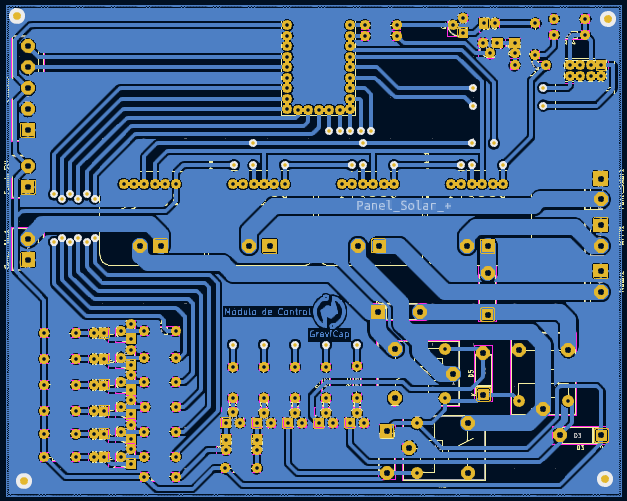
\includegraphics[width=0.8\linewidth]{Imagenes/Hardware/PCB.jpg}
                    \caption{PCB del Sistema de Control}
                    \label{fig:h1}
                \end{figure}

            \begin{figure}
                \centering
                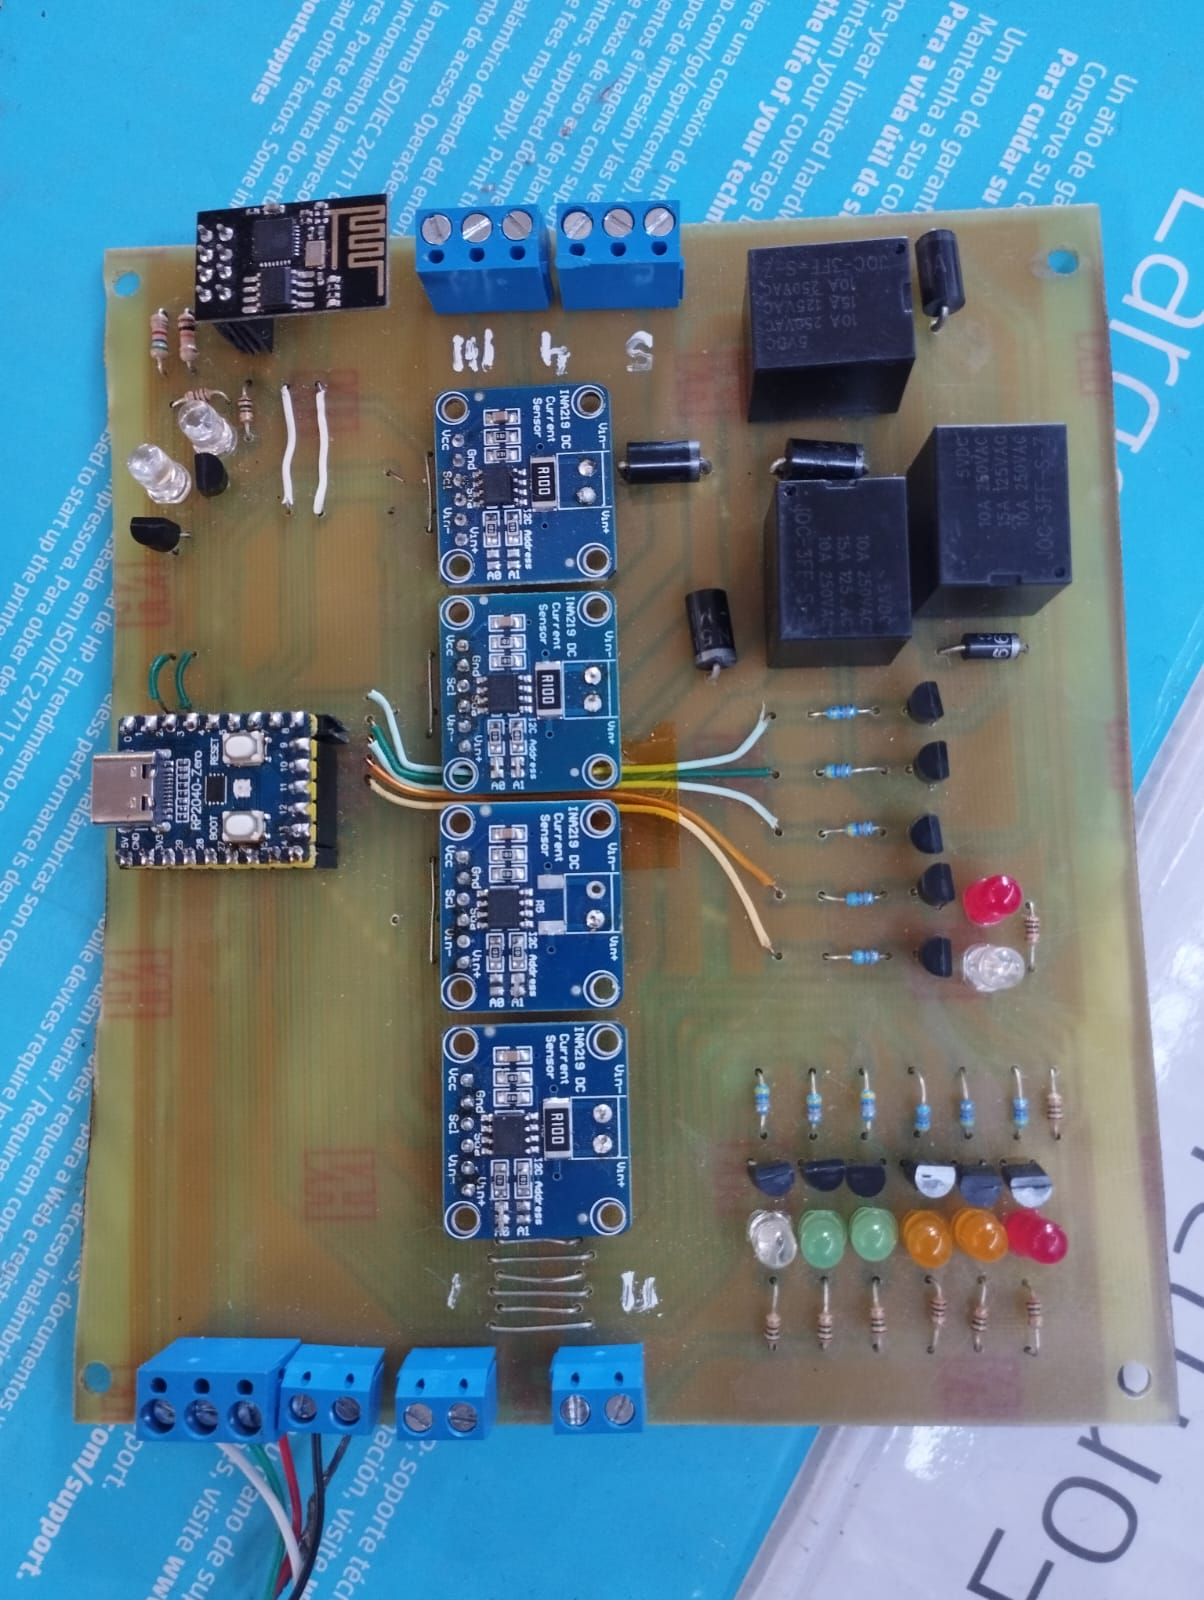
\includegraphics[width=0.5\linewidth]{Imagenes/Hardware/Finished.jpg}
                \caption{PCB finalizado del Sistema de Control}
                \label{fig:h2}
            \end{figure}